% Theta Gate -- submission deck (Alpaca AI Trading Agents Hackathon).
%
% Build:  make        (or: xelatex theta-gate.tex, twice)
% Output: theta-gate.pdf, 16:9.
%
% Deliberately depends only on what ships with TeX Live *basic*: beamer,
% tikz, xcolor, fontspec. No tcolorbox, no pgfplots, no plex package --
% this has to build on a teammate's machine and in CI without a tlmgr
% install anyone needs admin rights for. The equity chart and the
% architecture diagram are hand-drawn in tikz for the same reason.
%
% Fonts degrade rather than fail: IBM Plex if present (it is what
% docs/diagrams/*.html and app.py use), otherwise whatever sans the
% machine has. Never let a missing font break the build two days before
% a deadline.
%
% NUMBERS: every P&L figure lives in the "Results" frame and is marked
% \PLACEHOLDER until Thursday 3 Sep, when the book is flat and there is a
% settled number to report. Do not quote a P&L anywhere else in this file
% -- one number in one place is the only way it stays honest under edit.

\documentclass[aspectratio=169,10pt]{beamer}

\usepackage{fontspec}
\usepackage{tikz}
\usepackage{xcolor}
\usetikzlibrary{positioning,arrows.meta,calc,shapes.geometric}

% ---------------------------------------------------------------------------
% Brand -- lifted from docs/diagrams/architecture.html and app.py so the
% deck, the diagrams and the live demo read as one artifact.
% ---------------------------------------------------------------------------
\definecolor{ink}{HTML}{0B0D0F}
\definecolor{paper}{HTML}{F5F5F5}
\definecolor{accent}{HTML}{3F2AC1}
\definecolor{muted}{HTML}{5B5B5B}
\definecolor{soft}{HTML}{838BA0}
\definecolor{rule}{HTML}{DDDEE3}
\definecolor{win}{HTML}{1F7A5C}
\definecolor{loss}{HTML}{B3261E}

\IfFontExistsTF{IBM Plex Sans}{
  \setsansfont{IBM Plex Sans}[UprightFont=* Light, BoldFont=* SmBld]
}{
  \IfFontExistsTF{Helvetica Neue}{\setsansfont{Helvetica Neue}[UprightFont=* Light]}{}
}
\IfFontExistsTF{IBM Plex Mono}{\setmonofont{IBM Plex Mono}[Scale=0.86]}{
  \IfFontExistsTF{Menlo}{\setmonofont{Menlo}[Scale=0.82]}{}
}

\usetheme{default}
\usecolortheme{default}
\setbeamercolor{normal text}{fg=ink,bg=paper}
\setbeamercolor{frametitle}{fg=ink,bg=paper}
\setbeamercolor{structure}{fg=accent}
\setbeamercolor{itemize item}{fg=accent}
\setbeamercolor{itemize subitem}{fg=soft}
\setbeamerfont{frametitle}{size=\large,series=\bfseries}
\setbeamertemplate{navigation symbols}{}
\setbeamertemplate{itemize item}{\textcolor{accent}{\rule[0.28ex]{0.5em}{0.5pt}}}
\setbeamertemplate{itemize subitem}{\textcolor{soft}{\rule[0.28ex]{0.35em}{0.4pt}}}
\setlength{\parskip}{0.30em}
\setbeamersize{text margin left=1.3em,text margin right=1.3em}

% Eyebrow label above each frame title, plus a hairline under it.
\setbeamertemplate{frametitle}{%
  \vspace{0.4em}%
  {\usebeamerfont{frametitle}\usebeamercolor[fg]{frametitle}\insertframetitle}\par
  \vspace{0.18em}\textcolor{rule}{\rule{\textwidth}{0.4pt}}\par\vspace{0.29em}}

\setbeamertemplate{footline}{%
  \hfill\textcolor{soft}{\ttfamily\scriptsize
    theta gate\quad\insertframenumber\,/\,\inserttotalframenumber}\hspace{2em}\vspace{0.4em}}

% ---------------------------------------------------------------------------
% Helpers
% ---------------------------------------------------------------------------
\newcommand{\eyebrow}[1]{{\ttfamily\scriptsize\textcolor{soft}{\MakeUppercase{#1}}}\par\vspace{0.22em}}
\newcommand{\lead}[1]{{\large #1}\par\vspace{0.43em}}
\newcommand{\kbd}[1]{{\ttfamily\small\textcolor{accent}{#1}}}
\newcommand{\PLACEHOLDER}[1]{{\bfseries\textcolor{loss}{[#1]}}}

% A quiet bordered panel. tcolorbox is not in TeX Live basic, so this is
% a plain tikz node -- same look, no dependency.
\newcommand{\panel}[2][white]{%
  \begin{tikzpicture}
    \node[fill=#1,draw=rule,line width=0.4pt,inner sep=10pt,
          text width=\dimexpr\textwidth-24pt\relax,align=left] {#2};
  \end{tikzpicture}}

\newcommand{\stat}[3]{%
  \begin{minipage}[t]{#1}
    {\ttfamily\scriptsize\textcolor{soft}{\MakeUppercase{#2}}}\par\vspace{0.25em}
    {\LARGE #3}
  \end{minipage}}

\title{Theta Gate}
\author{}
\date{}

\begin{document}

% ===========================================================================
\begin{frame}[plain]
  \vspace{1.6cm}
  {\ttfamily\Large\textcolor{ink}{T\,H\,E\,T\,A\ \ G\,A\,T\,E}}

  \vspace{0.65em}
  {\LARGE An autonomous options agent that\\[0.15em]
   cannot place a trade it should not.}

  \vspace{1.01em}
  \textcolor{muted}{The model proposes a direction. Deterministic Python does everything else.\\
  A pure-function risk guard has the last word, and cannot be argued with.}

  \vfill
  {\ttfamily\scriptsize\textcolor{soft}{ALPACA AI TRADING AGENTS HACKATHON\quad\textbullet\quad 28 AUG -- 4 SEP 2026\quad\textbullet\quad PAPER TRADING}}
  \vspace{0.6cm}
\end{frame}

% ===========================================================================
\begin{frame}[t]{The tension nobody else had to resolve}
  \eyebrow{the problem}

  Alpaca shipped their paper-trading skills on \textbf{25 August} --- the day before this
  build started. Their own guidance requires a \textbf{human confirmation before every
  order}, and five operations demand it \emph{regardless} of the unattended-mode setting:

  \vspace{0.29em}
  \kbd{cancel\_all\_orders}\quad \kbd{close\_all\_positions}\quad \kbd{close\_position}\\
  \kbd{exercise\_options\_position}\quad \kbd{do\_not\_exercise\_options\_position}

  \vspace{0.65em}
  \panel{%
    \textbf{That is fundamentally incompatible with the autonomous agent this hackathon
    asks for.} A cron at 10:30 on a Tuesday has nobody to ask.}

  \vspace{0.43em}
  \textcolor{muted}{\itshape\small ``Every deployed path asserts paper at startup\ldots\ There is
  no operator watching to catch a wrong endpoint, and a live account returns the same
  response shape as a paper one.'' \normalfont\upshape--- Alpaca's own skill}
\end{frame}

% ===========================================================================
\begin{frame}[t]{Confirmation is two things wearing one name}
  \eyebrow{the idea}

  \lead{A human confirmation does \textbf{legibility} (showing what is about to happen) and
  \textbf{authority} (deciding whether it may).}

  Alpaca automates away the second whenever a human is absent, and replaces it with an
  assertion that fails closed. \textbf{Theta Gate does the same thing, with 21
  assertions instead of one.}

  \vspace{0.72em}
  \panel[white]{%
    \textbf{The one idea:} the LLM has no tools at all. Every write goes through
    deterministic Python. The proposer suggests a direction; it never picks a strike, sizes
    a position, or holds an order credential.

    \vspace{0.36em}
    The breach is \emph{not reachable} --- not merely forbidden by a prompt.}

  \vspace{0.43em}
  \textcolor{muted}{\small This is why the guard is pure functions with no I/O: it is the only
  component in the system holding a real decision.}
\end{frame}

% ===========================================================================
\begin{frame}[t]{Architecture}
  \eyebrow{one tick, every five minutes}
  \vspace{-0.2em}

  \centering
  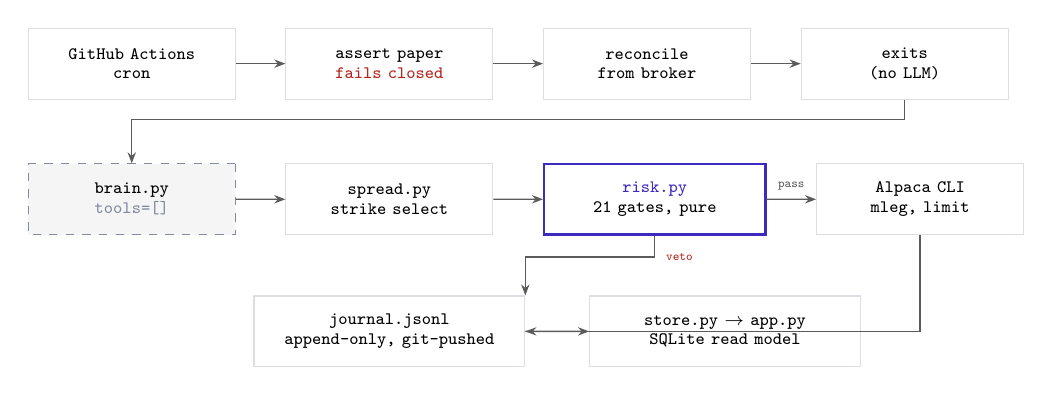
\begin{tikzpicture}[scale=0.9,transform shape,
      font=\ttfamily\scriptsize,
      box/.style={draw=rule,fill=white,line width=0.4pt,inner sep=6pt,
                  minimum height=1.0cm,text width=2.5cm,align=center},
      guard/.style={box,draw=accent,line width=0.9pt,text width=2.7cm},
      llm/.style={box,fill=paper,draw=soft,dashed},
      ar/.style={-{Stealth[length=4pt]},draw=muted,line width=0.5pt}]

    \node[box] (cron) {GitHub Actions\\cron};
    \node[box,right=0.7cm of cron] (paper) {assert paper\\\textcolor{loss}{fails closed}};
    \node[box,right=0.7cm of paper] (rec) {reconcile\\from broker};
    \node[box,right=0.7cm of rec] (exits) {exits\\(no LLM)};

    \node[llm,below=0.9cm of cron] (brain) {brain.py\\\textcolor{soft}{tools=[]}};
    \node[box,right=0.7cm of brain] (resolve) {spread.py\\strike select};
    \node[guard,right=0.7cm of resolve] (risk) {\textcolor{accent}{risk.py}\\21 gates, pure};
    \node[box,right=0.7cm of risk] (submit) {Alpaca CLI\\mleg, limit};

    \node[box,below=0.85cm of resolve,text width=3.4cm] (journal) {journal.jsonl\\append-only, git-pushed};
    \node[box,right=0.9cm of journal,text width=3.4cm] (dash) {store.py $\rightarrow$ app.py\\SQLite read model};

    \draw[ar] (cron) -- (paper);
    \draw[ar] (paper) -- (rec);
    \draw[ar] (rec) -- (exits);
    \draw[ar] (exits.south) -- ++(0,-0.28) -| (brain.north);
    \draw[ar] (brain) -- (resolve);
    \draw[ar] (resolve) -- (risk);
    \draw[ar] (risk) -- node[above,font=\ttfamily\tiny,text=muted]{pass} (submit);
    \draw[ar] (risk.south) -- ++(0,-0.30) node[right,font=\ttfamily\tiny,text=loss,xshift=1pt]{veto} -| (journal.north east);
    \draw[ar] (submit.south) |- (journal.east);
    \draw[ar] (journal) -- (dash);
  \end{tikzpicture}

  \vspace{0.5em}
  \raggedright\textcolor{muted}{\small The dashed box is the only non-deterministic component
  in the system, and it is the one with no network access, no credential, and no ability to
  write anything.}
\end{frame}

% ===========================================================================
\begin{frame}[t]{The LLM boundary, in full}
  \eyebrow{brain.py}

  \small

  \panel[white]{\ttfamily\small
  options = ClaudeAgentOptions(\\
  \hspace*{2em}system\_prompt=SYSTEM\_PROMPT, model=MODEL\_ID, max\_turns=1,\\
  \hspace*{2em}\textcolor{accent}{tools=[], allowed\_tools=[], mcp\_servers=\{\},}\\
  \hspace*{2em}\textcolor{accent}{strict\_mcp\_config=True, setting\_sources=[],}\\
  )}

  \vspace{0.65em}
  Zero tools. Zero MCP servers. One turn. No filesystem, user, or project settings.
  It sees only the same scalar market numbers already computed for the gates ---
  no chain, no news, no broker credential.

  \vspace{0.5em}
  It may return exactly five fields: \kbd{underlying}, \kbd{direction},
  \kbd{confidence}, \kbd{thesis}, \kbd{invalidation}.

  \vspace{0.5em}
  \textbf{Why not a read-only allowlist?} An allowlist still holds a network client and still
  depends on being maintained correctly forever. \kbd{tools=[]} cannot reach anything, and
  \kbd{strict\_mcp\_config=True} means a stray \kbd{.mcp.json} cannot quietly re-arm it.

  \vspace{0.36em}
  \textcolor{muted}{\small Any failure --- malformed JSON, schema violation, timeout, or a
  thesis that reads back an injected instruction --- produces no proposal, never a crash.}
\end{frame}

% ===========================================================================
\begin{frame}[t]{The guard}
  \eyebrow{risk.py --- pure functions, no I/O, time injected}

  \footnotesize
  \begin{columns}[T]
    \begin{column}{0.49\textwidth}
      \textcolor{soft}{\ttfamily\scriptsize ENVIRONMENT}
      \begin{itemize}\itemsep1pt
        \item paper asserted before \emph{every} order
        \item kill-switch file; account status; options level $\geq$ 3
      \end{itemize}
      \vspace{0.22em}
      \textcolor{soft}{\ttfamily\scriptsize REGIME (entry-only, never blocks an exit)}
      \begin{itemize}\itemsep1pt
        \item VIX $<$ 30 and VIX9D $<$ VIX3M
        \item $|$intraday move$| < 2\%$
        \item FOMC / CPI / PCE / NFP blackout
      \end{itemize}
      \vspace{0.22em}
      \textcolor{soft}{\ttfamily\scriptsize CONTRACT}
      \begin{itemize}\itemsep1pt
        \item both legs need delta \emph{and} IV --- the 0DTE guard
        \item $3 \leq$ DTE $\leq 5$; short leg $0.16 \leq |\delta| \leq 0.25$
        \item quote age $\leq$ 60s; spread $\leq 15\%$ of mid
      \end{itemize}
    \end{column}
    \begin{column}{0.49\textwidth}
      \textcolor{soft}{\ttfamily\scriptsize PRICE}
      \begin{itemize}\itemsep1pt
        \item credit within $\pm40\%$ of $0.8 \times$ short delta
        \item absolute floor: credit $\geq 10\%$ of width
        \item ATM IV $-$ 10d realised vol $\geq$ 1.0 point
      \end{itemize}
      \vspace{0.22em}
      \textcolor{soft}{\ttfamily\scriptsize SIZE AND EXPOSURE}
      \begin{itemize}\itemsep1pt
        \item max loss $\leq$ \$1{,}000; open risk $\leq$ \$3{,}000
        \item $\leq$ 2 open, $\leq$ 1 per underlying
        \item buying power $\geq$ \$25{,}000 \emph{and} $\geq 5\times$ max loss
      \end{itemize}
      \vspace{0.22em}
      \textcolor{soft}{\ttfamily\scriptsize DRAWDOWN}
      \begin{itemize}\itemsep1pt
        \item $-1\%$ on the day $\rightarrow$ no new entries
        \item equity $\leq$ \$98{,}000 $\rightarrow$ HALT, no new entries
      \end{itemize}
    \end{column}
  \end{columns}

  \vspace{0.58em}
  \panel{\small \textbf{First rejection wins and is final.} No gate is re-evaluated after a
  veto, and no LLM sits downstream of one. Every number lives in \kbd{governance.json},
  rendered verbatim on the dashboard beside the line \emph{``no LLM can write to this file''}.}
\end{frame}

% ===========================================================================
\begin{frame}[t]{The strategy, and its honest edge}
  \eyebrow{what it actually trades}

  \small

  \lead{Short credit vertical on SPY or QQQ. \$5 wide. 3--5 DTE. Short leg at 0.16--0.25
  delta. Two contracts, fixed, since 31 August.}

  \begin{columns}[T]
    \begin{column}{0.5\textwidth}
      \textcolor{soft}{\ttfamily\scriptsize WHY TWO LEGS, NEVER A CONDOR}\par
      Half the legs, half the fills to win. Roughly 10\% of eligible paper fills come back
      partial, and a 4-leg order that half-fills \emph{manufactures a naked short}.
      Non-negotiable.
      \vspace{0.43em}

      \textcolor{soft}{\ttfamily\scriptsize WHY NOT 0DTE}\par
      0DTE has no greeks and no IV, so a delta-targeting rule has no input at all. This is
      structural, not a preference.
    \end{column}
    \begin{column}{0.5\textwidth}
      \panel{%
        \textbf{There is no arithmetic edge, and we say so.}

        \vspace{0.29em}
        Sweeping every strike from 0.15 to 0.45 delta across five widths, expected value is
        \textbf{negative in every case} --- between $-\$4$ and $-\$8$ per contract, precisely
        the bid-ask cost. Delta \emph{is} the risk-neutral probability, so a fairly priced
        chain cannot yield edge by arithmetic.

        \vspace{0.29em}
        The only defensible claim is the \textbf{variance risk premium}: implied vol has
        historically exceeded realised. Real, thin, and \textbf{six sessions cannot measure
        it}.

        \vspace{0.3em}
        The LLM is a direction filter and a veto. It is not the edge.}
    \end{column}
  \end{columns}

  \vspace{0.36em}
\end{frame}

% ===========================================================================
\begin{frame}[t]{Three things live testing corrected}
  \eyebrow{one real spread, opened and closed, 26 august}

  \small

  \vspace{0.15em}
  \panel{%
    \textbf{1. The original credit gate would have vetoed every trade.}
    We specified credit/width of 0.20--0.45. Observed on SPY at 765.55, 7 DTE, short leg at
    $-0.197$ delta: net credit \textbf{0.60 --- a ratio of 0.120}. Widening makes it
    \emph{worse}, monotonically. Across the chain the real relationship is
    \textbf{credit/width $\approx 0.8 \times$ short delta}. Recalibrated to a relative test.}

  \vspace{0.4em}
  \panel{%
    \textbf{2. Margin held is the full width, not the max loss.}
    The fill consumed exactly \textbf{\$500} of options buying power on one \$5-wide
    contract --- $\text{width} \times 100 \times \text{qty}$ --- while max loss was \$443.
    Two different numbers; the buying-power gate used the wrong one.}

  \vspace{0.4em}
  \panel{%
    \textbf{3. A duplicate \kbd{client\_order\_id} is rejected, never duplicated.}
    Alpaca returns HTTP 422. That single verified fact is the entire idempotency mechanism
    --- it is what lets a crashed tick re-run safely with \emph{no database at all}.

    \vspace{0.3em}
    \textcolor{muted}{Every one of these was a plan that read fine and was wrong.}}
\end{frame}

% ===========================================================================
\begin{frame}[t]{Durability without a database}
  \eyebrow{what we deliberately did not build}

  \small

  The canonical design called for Postgres with row-level security, six credentialed roles,
  OIDC/Sigstore attestation, fenced distributed leases and hash-chained event sourcing.
  That is weeks of distributed-systems work. \textbf{We cut it, on the record, and said why.}

  \vspace{0.65em}
  \begin{columns}[T]
    \begin{column}{0.5\textwidth}
      \textcolor{soft}{\ttfamily\scriptsize WHAT REPLACED IT}
      \begin{itemize}\itemsep2pt
        \item \textbf{Idempotency from the broker.} A deterministic \kbd{client\_order\_id}, always looked up before submitting.
        \item \textbf{Concurrency} is one Actions \kbd{concurrency:} group --- a platform feature.
        \item \textbf{The broker is the source of truth}, refetched every tick.
        \item \textbf{The journal} is append-only JSONL, written \emph{before} the network call that might submit.
      \end{itemize}
    \end{column}
    \begin{column}{0.5\textwidth}
      \panel{%
        \textbf{SQLite, but only downstream.}

        \vspace{0.29em}
        The dashboard needs aggregates, so \kbd{store.py} replays the journal into SQLite
        with a \kbd{sha256} hash chain, making an edited history detectable.

        \vspace{0.29em}
        It is a pure \emph{function} of the journal --- rebuilt from line 1, gitignored,
        never authoritative. A binary \kbd{.db} in the git-publish path would collide with
        the one durability mechanism we actually have. JSONL merges; a database file
        does not.}
    \end{column}
  \end{columns}
\end{frame}

% ===========================================================================
\begin{frame}[t]{What the agent did}
  \eyebrow{results --- paper account, fresh, \$100,000}

  \small

  \vspace{0.36em}
  \stat{0.22\textwidth}{realised p\&l}{\PLACEHOLDER{P\&L}}\hfill
  \stat{0.22\textwidth}{trades closed}{\PLACEHOLDER{n}}\hfill
  \stat{0.22\textwidth}{win rate}{\PLACEHOLDER{\%}}\hfill
  \stat{0.22\textwidth}{max drawdown}{\PLACEHOLDER{\%}}

  \vspace{0.86em}
  \centering
  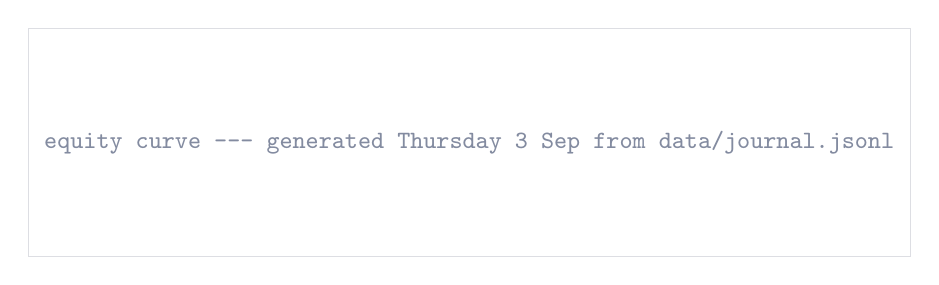
\begin{tikzpicture}
    \draw[draw=rule,line width=0.4pt,fill=white] (0,0) rectangle (11.2,2.9);
    \node[text=soft,font=\ttfamily\small] at (5.6,1.45)
      {equity curve --- generated Thursday 3 Sep from data/journal.jsonl};
  \end{tikzpicture}

  \vspace{0.65em}
  \raggedright
  \panel{\small \textbf{Every trade above was placed by the agent.} The account has never
  received a manual order --- not one, not even a test. Its history \emph{is} the evidence of
  autonomy, so every live experiment in this deck used a separate throwaway account.}
\end{frame}

% ===========================================================================
\begin{frame}[t]{What six sessions can and cannot show}
  \eyebrow{the part most decks leave out}

  \small

  \lead{The sample is \PLACEHOLDER{n} trades across six sessions. That is statistically
  nothing, and we are not going to claim otherwise.}

  \begin{columns}[T]
    \begin{column}{0.5\textwidth}
      \textcolor{soft}{\ttfamily\scriptsize WHAT THIS CANNOT DEMONSTRATE}
      \begin{itemize}\itemsep2pt
        \item That the strategy has edge. At $-0.197$ delta the breakeven win rate is 88\% against a risk-neutral 80\%.
        \item The sign of the P\&L. One 2\% adverse gap inside six sessions erases the book.
      \end{itemize}
    \end{column}
    \begin{column}{0.5\textwidth}
      \textcolor{soft}{\ttfamily\scriptsize WHAT IT CAN DEMONSTRATE}
      \begin{itemize}\itemsep2pt
        \item That the guard held: which gates fired, how often, and that no trade was placed outside them.
        \item That loss is capped by construction --- max loss is the width, fixed at entry. A dropped cron run cannot exceed it.
        \item That the agent ran unattended, reconstructable from a committed, hash-chained journal.
      \end{itemize}
    \end{column}
  \end{columns}

  \vspace{0.58em}
  \panel{\small \textbf{The number worth judging is not the P\&L. It is whether the risk
  guard held} --- and that is measurable at n~=~\PLACEHOLDER{n}, whereas edge is not.}
\end{frame}

% ===========================================================================
\begin{frame}[t]{Built, and what it cost}
  \eyebrow{engineering}

  \small

  \begin{columns}[T]
    \begin{column}{0.52\textwidth}
      \textcolor{soft}{\ttfamily\scriptsize THE SYSTEM}
      \begin{itemize}\itemsep2pt
        \item \kbd{risk.py} --- 21 gates, pure functions, no I/O, time injected
        \item \kbd{spread.py} --- deterministic strike selection and mleg construction
        \item \kbd{loop.py} --- one tick; recovery, reconcile, exits, entry, journal
        \item \kbd{brain.py} --- the single bounded model call
        \item \kbd{store.py} / \kbd{app.py} --- read model and live dashboard
      \end{itemize}
      \vspace{0.36em}
      \textcolor{soft}{\ttfamily\scriptsize THE INTEGRATION}\par
      Alpaca CLI for every broker call. No \kbd{alpaca-py}, by choice.
    \end{column}
    \begin{column}{0.44\textwidth}
      \panel{%
        \textbf{Nothing here is claimed untested.}

        \vspace{0.29em}
        Where a fact could be verified against the live API, it was --- the 422 on a
        duplicate order id, the margin arithmetic, the credit/delta curve, the
        \kbd{alpaca doctor --profile} flag that silently lies.

        \vspace{0.29em}
        Adversarial review passes over \kbd{loop.py} caught and fixed real defects ---
        including a zero-bid exit leg and an id-less order hit --- before any of it was
        trusted with an order.}
    \end{column}
  \end{columns}

  \vspace{0.5em}
  \textcolor{muted}{\small The honest failure mode: roughly 4:1 against --- about eight \$100
  wins per one \$800 loss. The gates cap the left tail; they do not change the sign of a week.}
\end{frame}

% ===========================================================================
\begin{frame}[plain]
  \vspace{2.2cm}
  {\ttfamily\large\textcolor{ink}{T\,H\,E\,T\,A\ \ G\,A\,T\,E}}

  \vspace{0.72em}
  {\LARGE The risk guard is what replaces\\[0.15em] the human confirmation step.}

  \vspace{0.72em}
  \textcolor{muted}{It is the thing you must build if you want autonomy without recklessness ---\\
  and it is the gap Alpaca's own tooling leaves open.}

  \vfill
  {\ttfamily\scriptsize\textcolor{soft}{PAPER TRADING ONLY\quad\textbullet\quad NO MANUAL ORDERS, EVER\quad\textbullet\quad FULL JOURNAL COMMITTED TO GIT}}
  \vspace{0.8cm}
\end{frame}

\end{document}
